\chapter{Hierarchical orchestration}
\label{ch:Hierarchical Orchestration}

\paragraph{} The orchestration of a network service in a MANO is one of the responsibilities of NFVO. The VNFM along with NFVO are responsible for managing the VNF instances and its lifecyle. To achieve end-to-end provisioning, a single MANO platform is not feasible in most of the cases. 
A multi-domain NFVI that allows interaction of multiple administrative domains at different levels is required.
To satisfy the requirements of a multi-domain, multi-vendor, multi-technology interoperability environments, the orchestration of network services can be done in a hierarchical fashion or in a peer-to-peer fashion. \cite{munoz2018hierarchical}

\paragraph{} In a peer-to-peer orchestrating model, the MANOs are interconnected to each other in an arbitrary fashion to provide end-to-end network services. This model is preferred when
there is no cross-domain control or cross-domain visibility is required, thus limiting the scaling
possibilities of a MANO. \cite{munoz2018hierarchical}


\paragraph{}In a hierarchical orchestrating model, one of the MANO acts as a global orchestrator to the
underlying MANO with a parent/child hierarchy. This architecture uses a common API between
the parent MANO and child MANOs, hence maintaining a good overview of the global system. Each hierarchical level deals with a minimum of one orchestrator. The orchestrator at any given level is managed by the higher level orchestrator. Some of the factors influencing hierarchical orchestration are the geographical spread and placement of MANOs across regions, scalability constraints of peer-to-peer architectures, different administrative requirements from the operators with different layers of abstraction. This architecture is preferred because of its broader scope of network services from the lower MANOs and also for better abstraction. The number of levels of hierarchy in this type of orchestration is based on the geographical region and network domain. The hierarchical levels are also based on abstraction required for the provisioning of network services \cite{munoz2018hierarchical}.


\paragraph{}The overall orchestration of the hierarchical model is split based on its geographical domains known as execution zones (EZ). The splitting of EZ further is based on the geographical area the domain covers. The grouping of few data centers which are geographically close for one execution zone. The number of data centers in a region is proportional to the number of execution zones required for the region. Supposedly, here, the whole world is split into 11 execution zones based on their geographical regions like, Western Europe (EUW), Eastern Europe (EUE), Central Asia (ASC), Southern Asia (ASS), Pacific Asia (ASP), Africa (AFR), Northern North America (NAN), Southern North America (NAS), Eastern South America (SAE), Western South America (SAW) and Oceania (OCE). Considering one of the regions, like Western Europe (EUW), it is further split into lower levels based on the resolution domains (RD). The lower levels can further be split based on the granularity of orchestration required\cite{maini2016hierarchical}.

\paragraph{}Each RDs constitutes number of EZs located at a specific location for users. Here, as an example, the first level(level 0)  split is based on 3 resolution domains, RD1, RD2, RD3. With a limited visibility of EZs for the high level orchestrator makes a placement decision. The RDs are divided based on local-local requests of a EZ, remote-local requests of EZ, and local-remote requests of EZ. The next level of split is influenced by the scalable property of orchestrators in first level split \cite{maini2016hierarchical}.

\begin{figure}
	\centering
	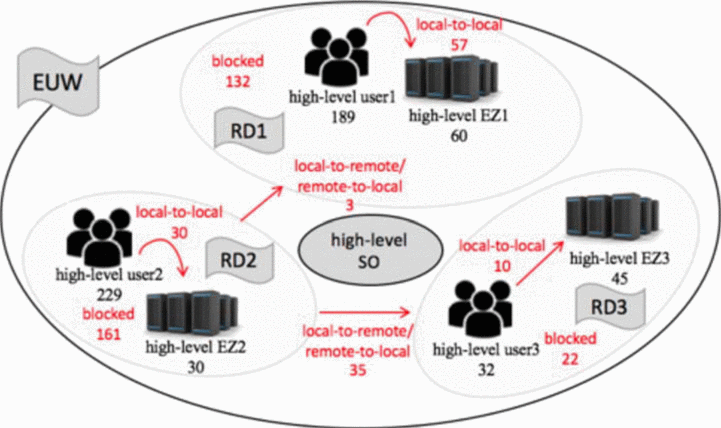
\includegraphics[width=0.7\linewidth]{figures/HO}
	\caption{An example of the placement decision made by the high-level orchestrator \cite{maini2016hierarchical}}
	\label{fig:ho}
\end{figure}

Thus, the above investigation of MANO scalability can infer the conclusions about optimal number of MANOs in such a system and also the optimal number of hierarchical levels. Considering the above example, the MANOs are initially placed in 3 RDs and that forms the first level of hierarchy. The number of MANOs and the level of hierarchy can increase further depending on the user requests in that location. When there is a demand for more number of MANOs to complete the service requests. The existing MANOs are designed to scale more MANOs using service replication/service migration techniques in a hierarchical fashion. 

\paragraph{}In the further chapters, we discuss about the SCrAMbLE plug-in architecture. This plug-in could be installed in SONATA/OSM MANO to make use of the services that is developed by Translator, Splitter and Adaptor. For the ease of plug-in development, we choose the top most MANO to be a SONATA(phishahang) MANO. Considering the same example of EUW region, 3 of the SONATA MANOs could be placed in 3 different RDs intially. These MANOs depending on the service requests will call OSM MANOs using the Adaptor services. When there is a situation when all the 3 MANOs reach a threshold where in they can not serve any more requests, additional MANOs are installed with a load balancer to further scale MANO using service replication techniques. The scaled(child) MANOs are also installed with SCrAMbLE plug-in and the same services can be made use to serve more requests. 
The scaling of any MANOs is handled by a component called scalability manager. This could be a part of MANO. We do not discuss the implementation details of the scalability manager at this point as it is still a work in progress.
